\def\thisdir{instrument/optics/}

\begin{center}
\section{Studies of the Optics for the Wide-Field Near-IR Imager and
 Multi-object Spectrograph
\label{sec:inst_optics}}
\vspace{0.5cm}

\noindent
\large
%% authors
{\bf T. Yamamuro$^{1}$, K. Motohara$^{2}$, I. Iwata$^{3}$ and Subaru
Telescope Next-Gen AO Instrument sub-working group}\\
$^1$ Optocraft
$^2$ Institute of Astronomy, University of Tokyo
$^3$ Subaru Telescope, National Astronomical Observatory of Japan
\vspace{0.5cm}

\end{center}

Here we summarize results of studies made by Dr. Yamamuro (Optcraft).
Document Number: CP0046--11--RP001 (w/o FoV split), CP0046--12--RP001 (w
FoV split).

\subsection{Optical Design without FoV Split}

First we studied how wide field of view can be achieved at the
Cassegrain focus of Subaru Telescope with the following conditions:

\begin{itemize}
 \item Single set of optics can be used (i.e., no FoV split is
       considered).
 \item We consider a near-infrared camera and spectrograph. Wavelength
       range is from 0.8$\mu$m to 2.5$\mu$m. The optics will be cooled
       down to about 100K.
 \item The target image quality is to achieve FWHM $<0.15''$ over the
       entire FoV in all of $J$, $H$, $K$-bands.
 \item The focal plane of the instrument should be flat so that we can
       achieve the above image quality by using science detectors with
       flat pixel arrays.
 \item The use of Teledyne H4RG (15$\mu$m pixel size) is assumed.
 \item The sizes of optical components should be feasibile; for example,
       the maximum size of components made of CaF$_2$ and BaF$_2$ should
       be less than 40cm.
\end{itemize}

We examined the two cases on the telescope parameters; (A) the case we
use the existing optical parameters of Subaru Telescope and (B) the case
with new parameters for the secondary mirror and also that the shape of 
primary mirror can be adjusted within the range of the stroke which the
existing mirror actuators are achievable.

Also, we should consider the necessity of field flatner for the
telescope focus. In order to achieve multi-object spectroscopy (MOS), we
need to insert a mask with slitlets at the telescope focus. Since the
Cassegrain focal plane has a curvature, in order to enable the use of
flat MOS mask, we need to insert field flatning lens(es). For the case
A, we show both the case with and without field flatner.

\subsubsection{A. Cases in which Subaru Telescope optical parameters are
   not changed}

Here we show the simplest case where there is no change in telescope
parameters and no field flatner is included.
Fig.\ref{fig:optcraft_fig01} is the optical layout. It consists of nine
collimator lenses and seven camera lenses. Lense materials are CaF$_2$, 
BaF$_2$, Fused silica, and ZnSe.The last lens of the camera section is
aspherical. 

\begin{figure}[!ht]
\centerline{
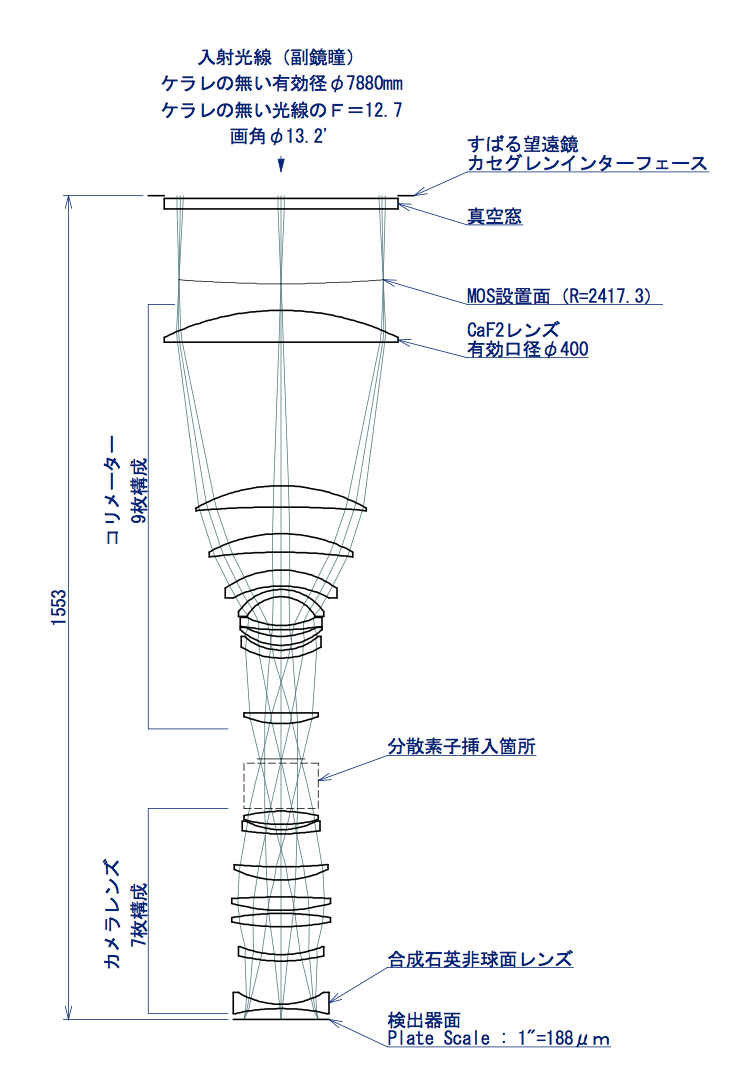
\includegraphics[width=120mm]{\thisdir figs/optcraft_fig01.eps}
}
\caption{Optical layout for Case A: no change in the telescope
 parameters. The case without field flatner.
}
\label{fig:optcraft_fig01}
\end{figure}

The field of view is determined so that the size of effective beam for
the largest lens is within $\phi$400mm, and in this solution it is 
$\phi 13.2'$. The effective diameter of the primary mirror is 
$\phi 7.88$m to achieve the above FoV at the secondary mirror pupil and
to block the light outside of the primary mirror (physical size 
$\phi$8.2m). Since this layout does not include field flatner, the
telescope focal plane has a curvature, and there is astigmatism.

The spot diagram at the position of the MOS mask (with a radius of
curvature of 2417.3mm) is shown in
Fig.~\ref{fig:optcraft_fig02}(left). The degradation of the image toward
the edge of FoV ($\sim 0.2''$ at the edge) is due to astigmatism. 
In this case the slit width at the edge should be adjusted to this image
quality. 
Fig.~\ref{fig:optcraft_fig02}(right) shows the size of distortion at the
position of the MOS mask.

\begin{figure}[!ht]
\centerline{
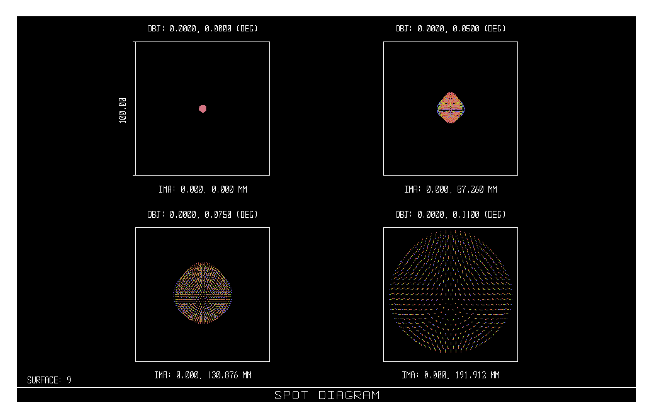
\includegraphics[width=100mm]{\thisdir figs/optcraft_fig02.eps}
 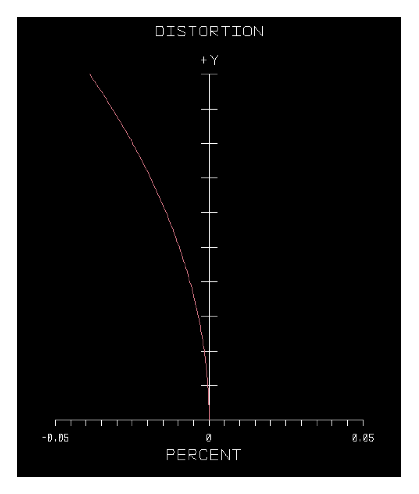
\includegraphics[width=60mm]{\thisdir figs/optcraft_fig03.eps}
}
\caption{(Left) Spot diagram at the position of the MOS mask with a
 curvature radius of 2417.3mm for a configuration shown in 
Fig.\ref{fig:optcraft_fig01}. Spot diagrams with wavelengths from
 0.8$\mu$m to 2.5$\mu$m are shown altogether, as wavelength dependence
 is small. (Right) distortion at the
 position of the MOS mask. The value is $-0.04$\% at the edge.
}
\label{fig:optcraft_fig02}
\end{figure}

The spot diagram and distortion at the position of the detectors are
shown in Fig. \ref{fig:optcraft_fig04}. All FWHM values are smaller than
the target FWHM (0.15$''$) except the case with 0.8$\mu$m
at the edge ($6.6'$) in which the FWHM is slightly larger than
0.15$''$. However, the distortion is large; at the edge it is 
$-6.3$\%.

\begin{figure}[!ht]
\centerline{
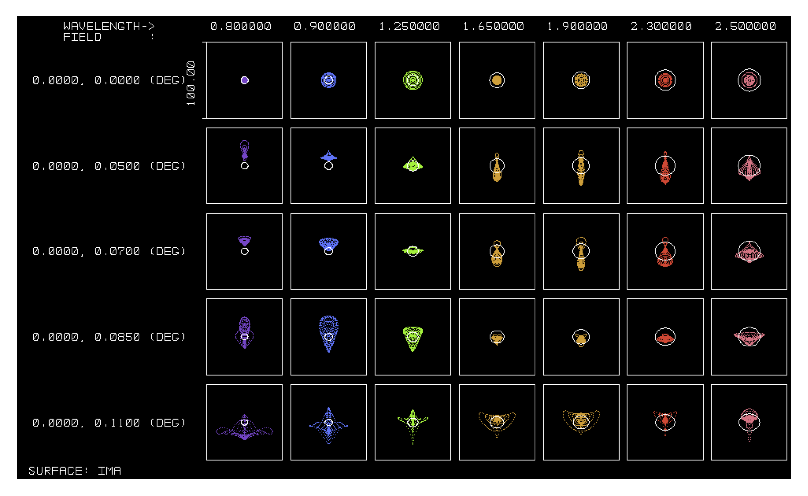
\includegraphics[width=120mm]{\thisdir figs/optcraft_fig04.eps}
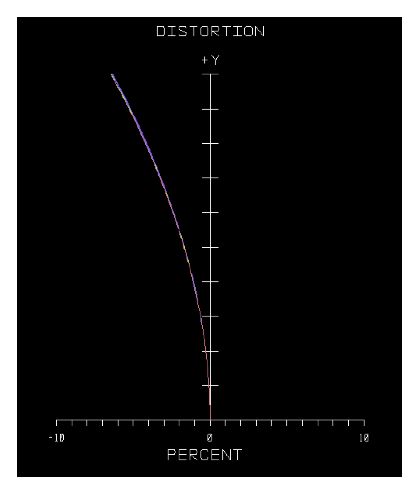
\includegraphics[width=60mm]{\thisdir figs/optcraft_fig05.eps}
}
\caption{(Left) Spot diagram at the position of the detectors for a
 configuration shown in Fig.\ref{fig:optcraft_fig01}.
Five positions from 0$'$ (center) to 6.6$'$ (edge) are shown along the
 vertical axis, and the cases with wavelengths from 0.8$\mu$m to
 2.5$\mu$m are plotted along the horizontal axis. 
The box size is 100$\mu$m which corresponds to 0.53$''$.
(Right) Distortion at the position of the detectors.
}
\label{fig:optcraft_fig04}
\end{figure}


We also evaluated the performance in spectroscopy. As a preliminary
analysis, here we only examined the image quality in spectroscopy in the
range 0.8--2.5$\mu$m without order-sorting.
Fig.~\ref{fig:optcraft_fig06} shows the positions of images in
spectroscopy as a function of wavelength.
Here we assume a fused silica grism with 160 grooves/mm, blaze angle 
34$\circ$\footnote{In section ** we examine more details of various
grisms}.
Fig.~\ref{fig:optcraft_fig07} is the spot diagram. Image qualities at
the shorter and longer wavelength edges and at the edge of FoV is not
good; in 2.5$\mu$m and at $6.6'$ from the center the RMS spot diameter
is $0.22''$. However, it is $0.17''$ at $5.5'$ from the center, and
at the other positions the image quality meets the goal.

\begin{figure}[!ht]
\centerline{
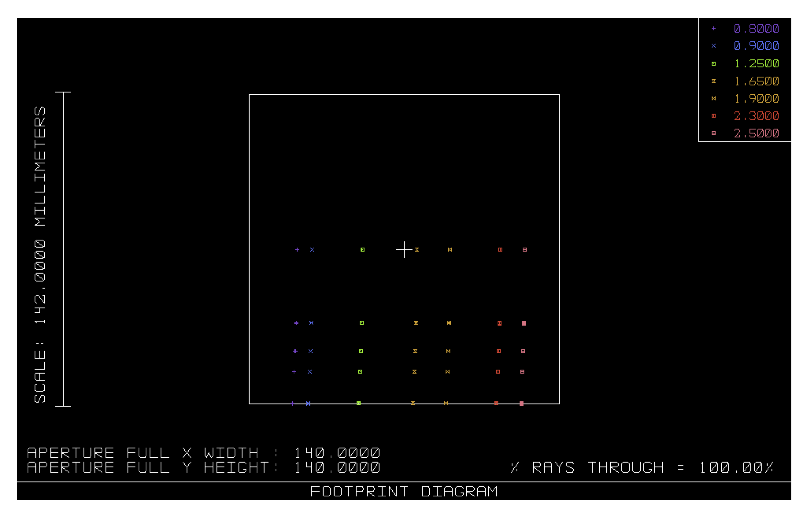
\includegraphics[width=120mm]{\thisdir figs/optcraft_fig06.eps}
}
\caption{Spectroscopic image positions for a configuration shown in Fig.~\ref{fig:optcraft_fig01}.
}
\label{fig:optcraft_fig06}
\end{figure}

\begin{figure}[!ht]
\centerline{
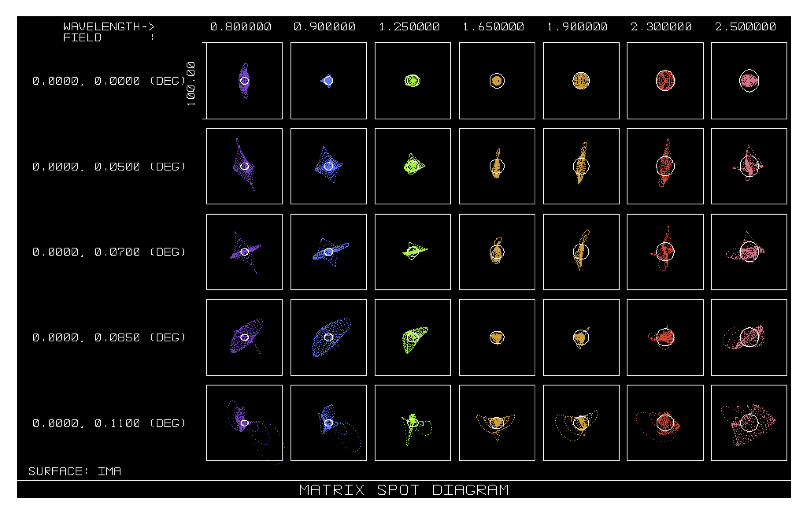
\includegraphics[width=120mm]{\thisdir figs/optcraft_fig07.eps}
}
\caption{Spot diagram for spectroscopy with a configuration shown in
 Fig.~\ref{fig:optcraft_fig01}.}
\label{fig:optcraft_fig07}
\end{figure}





\subsubsection{B. Cases in which Subaru Telescope optical parameters are
   changed}


\subsection{Optical Design with FoV Split}

\subsubsection{Case A: secondary mirror parameter is the same as
   existing one}

\subsubsection{Case B: secondary mirror parameter is modified}


